\chapter{Criação de Base}
\label{cap:banco}
Este capítulo tem como objetivo contextualizar o leitor na Rede Social Reddit,
apresentar o conteúdo selecionado para importação na base de dados e a forma na
qual este conteúdo foi extraído para a base de dados.
\section{Rede Social Reddit}
\label{cap:Reddit}

O \textit{website} Reddit teve seu início em 2005 como um agregador de
conteúdo e atualmente é o vigésimo terceiro \textit{website} mais acessado na
internet e o sétimo mais acessado nos Estados Unidos da América \cite{alexa}.
Os seus usuários do Reddit podem enviar \textit{links} para conteúdos externos
ao Reddit ou também mensagens de texto. A partir desse conteúdo enviado, os seus usuários
podem votar para cima (\textit{upvote}) ou para baixo \textit{downvote},
influenciando na posição do conteúdo no \textit{website}. Além de votar no conteúdo, seus usuários podem enviar comentários como
forma de expressar sua opinião.

O conteúdo do Reddit é distribuído em \textit{subreddits} que funcionam como
comunidades que abordam certos assuntos. Os usuários podem se inscrever nesses
\textit{subreddits}, recebendo as atualizações na sua página inicial. Dentre os
\textit{subreddits} destacam-se:


\begin{itemize}
  \item \textit{/r/AskReddit}: Utilizado para fazer perguntas gerais para
  outros usuários. Esse \textit{subreddit} possui atualmente 16.941.544 de inscritos.
  \item \textit{/r/worldnews}: Possui as notícias do mundo. Conta, atualmente,
  com 16.570.606 de inscritos.
  \item \textit{/r/IAmA}: IAmA é um estilização de 'I am a' ('Eu sou um').
  A partir desse \textit{subreddit} os usuários podem fazer perguntas ao criador
  de um determinado tópico. Esse \textit{subreddit} possui 16.941.544 de
  inscritos.
\end{itemize}

% Dentre esses \textit{subreddits} podemos destacar alguns dos tópicos mais
% acessados no ano de 2016:
% 
% \begin{itemize}
%   \item \textit{/r/IAmA} - \textit{We're NASA scientists \& exoplanet experts.
%   Ask us anything about today's announcement of seven Earth-size planets
%   orbiting TRAPPIST-1!} - Tópico de perguntas e respostas com cientistas da
%   NASA após a descoberta dos planetas que orbitavam a estrela TRAPPIST-1.
%   \item \textit{/r/IAmA} - \textit{I’m Bill Gates, co-chair of the Bill \&
%   Melinda Gates Foundation. Ask Me Anything.} - Tópico de perguntas e respostas com Bill Gates.
%   \item \textit{/r/worldnews} - \textit{Fidel Castro is dead at 90.} - Link para
%   anúncio da morte de Fidel Castro.
%   \item \textit{/r/AskReddit} - \textit{[Serious]South Koreans of Reddit, how
%   did they teach you about the existence of North Korea in School when you were
%   young?serious replies only} - Tópico perguntando para os usuários sul coreanos
%   como que foi ensinado para eles sobre a existência da Coreia do Norte.
% \end{itemize}

% A identificação de padrões de sentimentos expressos por determinados grupos
% dessa comunidade, se faz útil visto que a partir dessa avaliação é possível construir
% ferramentas que apoiam decisões tanto de um ponto de vista político, como por
% exemplo, entender qual é a opinião sobre um determinado assunto de um conjunto
% de eleitores, tanto quanto um ponto de vista de negócios, para entender qual a
% opinião dos consumidores de um produto, ou de seu competidor, a respeito de um
% determinado assunto.

\section{Extração de Dados}
\label{cap:Extracao}

Para a extração dos dados e criação da base foi
criado um \textit{crawler} ou robô de navegação. Esse robô tem como objetivo a navegação
automática no conteúdo web do Reddit, extraindo os dados referentes a tópicos e
a comentários e persistindo esses em um banco de dados.

O \textit{Crawler} foi escrito na linguagem Java. A Figura \ref{fig:crawler} representa a
arquitetura utilizada para desenvolvimento deste software.

\begin{figure}[htbp]
\centering
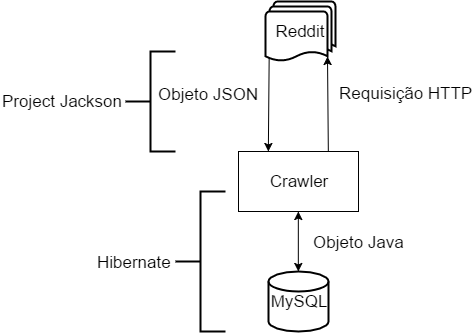
\includegraphics[height=225px]{imagens/arquitetura.png}
\caption{Arquitetura do \textit{Crawler}}
\label{fig:crawler}
\end{figure}

A partir de um \textit{link} para um tópico, o software tem como tarefa, a
extração e pesquisa de dados relacionados com o tópico em questão. Isso se faz
da seguinte forma, primeiramente, é enviada uma requisição para o \textit{link}
utilizando o sufixo ``.json'' (Exemplo: https://www.reddit.com/r/iama.json), a
partir dessa requisição, o \textit{website} retorna um objeto \ac{JSON}.

Como o \ac{JSON}, retornado pelo \textit{website}, possui 68 campos que assim
como seus tipos de dados, não se encontram em nenhuma documentação, foi utilizado o \textit{website}
jsonschema2pojo\footnote{http://www.jsonschema2pojo.org/} para mapear o \ac{JSON} retornado em um
objeto Java. Esse \textit{website} tem como objetivo a conversão de um esquema \ac{JSON} ou o próprio \ac{JSON} para um \ac{POJO} ou Os Singelos Clássicos Objetos Java, permitindo
o \textit{download} da classe para utilização, já com as anotações utilizadas na
biblioteca Jackson.

A partir deste objeto Java, foi utilizado o \textit{framework} Hibernate para a
criação do banco de dados, assim como persistência destes. O Hibernate mapeia essa
entidade junto ao banco de dados, neste caso, MySQL.

Para criação das tabelas do esquema do banco de dados, o próprio Hibernate
efetua essa na inicialização do servidor.

A execução do \textit{Crawler} funciona da seguinte forma, é enviada
uma requisição para o \textit{website} através da URL do tópico em questão com o
sufixo ``\textit{.json}'' no final. O \textit{website} retorna um
\textit{JSON} com os dados referentes ao tópico solicitado e aos comentários
deste tópico. Este objeto \ac{JSON} é convertido em um \ac{POJO} através da
biblioteca Jackson e persistida no banco de dados através do \textit{framework}
Hibernate.

\section{Tópicos Selecionados}

Para análise de sentimentos e comparação dos resultados obtidos, foram
selecionados 15 tópicos que apresentam o maior número de comentário de
determinados \textit{subreddits} o período do último ano até a data atual. Os 15
tópicos encontram-se distribuídos em diferentes assuntos, que são: cenário político nacional,
cenário político internacional e tópicos diversos:

No que diz respeito a tópicos relacionados com ao cenário político nacional, os
tópicos escolhidos foram:

\begin{itemize}
  \item
  \textit{Brazil Seeks To Copy U.S. Gun Culture ``to allow embattled
  citizens the right to defend themselves from
  criminals''}: encontra-se disponível em 
  \url{https://www.reddit.com/r/worldnews/comments/36ny58/brazil_blogger_known_for_reporting_on_corruption/}
  e refere-se a intenção do Brasil de copiar a cultura de porte de armas dos
  Estados Unidos da América.
  \item
  \textit{Brazil descends into chaos as Olympics looms}: encontra-se disponível em 
  \url{https://www.reddit.com/r/worldnews/comments/4bqcc3/brazil_descends_into_chaos_as_olympics_looms/}
  e refere-se ao caos olímpico no Brasil.
  \item
  \textit{Plane carrying Brazil Supreme Court judge crashes into sea}:
  encontra-se disponível em
  \url{https://www.reddit.com/r/worldnews/comments/5oyz3b/plane_carrying_brazil_supreme_court_judge_crashes/}
  e refere-se a queda do avião no qual o ministro Teori Zavascki estava abordo.
  \item
  \textit{Brazil passes Internet governance Bill: Brazil has made history with
  the approval of a post-Snowden Bill which sets out principles, rights and
  guarantees for Internet users.}: encontra-se disponível em
  \url{https://www.reddit.com/r/worldnews/comments/21f3as/brazil_passes_internet_governance_bill_brazil_has/}
  e se refere a aprovação do Marco Civil da Internet.
  \item
  \textit{FIFA generated more than \$4 billion in sales from the 2014 World Cup,
  and is Giving Brazil \$100 Million After The Country Spent \$15 Billion On The
  World Cup}: encontra-se disponível em
  \url{https://www.reddit.com/r/worldnews/comments/2t65ql/fifa_generated_more_than_4_billion_in_sales_from/}
  e se refere a diferença entre o lucro obtido pelo Brasil na Copa do Mundo de
  2014 e o que foi gasto.
 
\end{itemize}

Já os tópicos escolhidos que encontramos relacionados com a política
internacional foram:
\begin{itemize}
  \item
  \textit{2.6 terabyte leak of Panamanian shell company data reveals "how a
  global industry led by major banks, legal firms, and asset management companies
  secretly manages the estates of politicians, Fifa officials, fraudsters and
  drug smugglers, celebrities and professional
  athletes."}.: encontra-se disponível em
  \url{https://www.reddit.com/r/worldnews/comments/4d75i7/26_terabyte_leak_of_panamanian_shell_company_data/}
  e aborda o vazamento de uma sociedade de advogados panamenha.
  \item
  \textit{Fidel Castro is dead at
  90.}: encontra-se disponível em
  \url{https://www.reddit.com/r/worldnews/comments/5exz2e/fidel_castro_is_dead_at_90/}
  e aborda a morte de Fidel Castro.
  
  \item
  \textit{Donald Trump to strip all funding from State Dept team promoting
  women's rights around the world - Leaked plan comes as First Daughter Ivanka
  defends her father's record with women}: encontra-se disponível em
  \url{https://www.reddit.com/r/worldnews/comments/67ivae/donald_trump_to_strip_all_funding_from_state_dept/}
  e aborda a decisão de Donald Trump de remover fundos de promoção ao direito
  das mulheres.
  
  \item
  \textit{Manchester Arena 'explosions': Two loud bangs heard at MEN Arena}:
  encontra-se disponível em
  \url{https://www.reddit.com/r/worldnews/comments/6cqdye/manchester_arena_explosions_two_loud_bangs_heard/}
  e aborda o atentado terrorista ocorrido em Manchester em 23 de Maio de 2017.
  
  \item
  \textit{Sweden asks the U.S. to explain Trump comment on
  Sweden}: encontra-se disponível em
  \url{https://www.reddit.com/r/worldnews/comments/5uzetf/sweden_asks_the_us_to_explain_trump_comment_on/}
  e aborda os comentários feitos por Donald Trump sobre a Suécia.
  
  \item\textit{“Canada will welcome you,” Trudeau invites refugees as Trump bans
  them}: encontra-se disponível em
  \url{https://www.reddit.com/r/worldnews/comments/5qqa51/canada_will_welcome_you_trudeau_invites_refugees/}
  e aborda a decisão do Canada de receber refugiados enquanto Donald Trump bani
  eles de entrarem nos Estados Unidos da América.
\end{itemize}

Tópicos diversos.
\begin{itemize}
  \item
  \textit{I’m Bill Gates, co-chair of the Bill \& Melinda Gates Foundation. Ask
  Me Anything.}: encontra-se disponível em
  \url{https://www.reddit.com/r/IAmA/comments/5whpqs/im_bill_gates_cochair_of_the_bill_melinda_gates/}
  e refere-se a perguntas e respostas ao Bill Gates.
  \item
  \textit{Hey, it's Lars from Metallica. AMA}: encontra-se disponível em
  \url{https://www.reddit.com/r/IAmA/comments/1wl9ic/hey_its_lars_from_metallica_ama/}
  e aborda perguntas e respostas ao vocalista da banda Metallica.
  
  \item
  \textit{I'm the CEO of Renault and Nissan and we're making autonomous driving
  vehicles happen by 2020. Ask me anything!}: encontra-se disponível em
  \url{https://www.reddit.com/r/IAmA/comments/2s7obx/im_the_ceo_of_renault_and_nissan_and_were_making/}
  e aborda perguntas e respostas ao diretor executivo da Renault e Nissan.
  
  \item
  \textit{I am Julian Assange founder of WikiLeaks -- Ask Me Anything}:
  encontra-se disponível em
  \url{https://www.reddit.com/r/IAmA/comments/5n58sm/i_am_julian_assange_founder_of_wikileaks_ask_me/}
  e aborda perguntas e respostas ao Julian Assange, fundador do
  \textit{WikiLeaks}.
  
\end{itemize}


A partir destes tópicos selecionados, o conteúdo, o usuário de criação e número
de \textit{upvotes}. Destaca-se que só foram extraídos comentários
em resposta ao tópico em questão, comentários em resposta a outros comentários
foram desconsiderados uma vez que esses podem não estar relacionados com o
tópico em questão, tornando inválida ou prejudicando a análise de sentimento.


\chapter{Conclusão Parcial}

Como visto, o \ac{NLP} tem como objetivo a analise de linguagem natural, seja
essa escrita ou falada. Dentre diversas tarefas que ela executa, uma delas é a
análise de sentimentos, a qual se faz útil visto que cada vez
mais as pessoas se comunicam através de redes sociais, gerando um grande volume
de dados. A análise e quantificação da opinião expressa por esses dados, seja
por fins políticos, comerciais ou quaisquer outros, se torna díficil quando
feita de forma manual por sua quantidade de dados.

Através do estudo realizado, foram encontrados dois métodos de \ac{NLP}
distintos, métodos simbólicos, os quais se baseiam em regras, como por exemplo o
Método de Brill para análise léxica e estatísticos, como por exemplo a
utilização de Modelos de Markov, que utilizam aprendizado supervisionado. Dentro
da área do \ac{NLP} de análise de sentimentos, através da literatura, foram
verificados os métodos estatísticos \ac{SVM}, \ac{MaxEnt} e Naive Bayes, os quais apresentam
características e assertividade similar, a partir desses três foi
selecionado o método Naive Bayes para estudo e comparação com um método
simbólico. O método simbólico escolhido para estudo e comparação foi o
\ac{VADER}, visto que foi desenvolvido específicamente para o funcionamento em
redes sociais.
 
Através da literatura, foi verificado que o método \ac{VADER} se mostra superior
ao Naive Bayes na utilização para a análise de sentimentos nas avaliações de
produtos da Amazon, editoriais do New York Times e mais importante, na análise
de \textit{Tweets} da rede social Twitter. A justificativa para isso, se dá ao
fato de métodos estatísticos necessitarem de um \textit{training set}
especializado para obter resultados similares ou superiores aos métodos
simbólicos. Portanto, foi optado pelo método \ac{VADER}, visto que a não
especialização do \textit{training set} impactaria na assertividade da análise
de sentimentos e a especialização de um \textit{training set} para cada tema
distinto se faz inviável devido a quantidade de temas abordados pela rede social
Reddit. 

Para implementação do método \ac{VADER} foram verificadas diversas
ferramentas, porém, somente o \ac{NLTK} apresentou uma implementação deste,
visto que a utilização deste \textit{framework} facilitaria a execução da
análise de sentimentos, não só por já conter a implementação do \ac{VADER}, mas
também por conter outras implementações relacionadas com o \ac{NLP}, foi optada
pela utilização deste.
 
Por fim, se fez necessária a criação de uma base de dados para armazenar os
dados disponibilizados pelo Reddit, para isso, foi utilizado um banco de
dados MySQL, o qual através de uma ferramenta desenvolvida utilizando a
linguagem Java, elabora requisições para o Reddit e
persiste as respostas obtidas no formato JSON através da biblioteca
Hibernate. 

Através da base de dados criada, assim como o \ac{NLTK}, deverá ser possível
efetuar a análise de sentimentos na rede social Reddit com o objetivo de
encontrar padrões entre usuários, comunidades e opiniões.

\section{Atividade e Cronograma do TCC II}

Atividades a serem desenvolvidas para a conclusão do TCC II:
\begin{enumerate}
\item Implementação do software de Processamento de Linguagem Natural para a
análise de sentimentos na base de dados criada.
\item Análise dos resultados obtidos.
\item Redação da monografia TCC II.
\item Apresentação do TCC II.
\end{enumerate}

As atividades apresentadas podem ser observadas através da Tabela
\ref{tab:tcc2}.
\renewcommand{\arraystretch}{2}
\newcolumntype{Y}{>{\centering\arraybackslash}X}
\begin{table}[!htb]
\begin{tabularx}{0.9\textwidth}{Y|Y|Y|Y|Y|Y|Y|Y|Y|Y|Y|}
& \multicolumn{2}{|c|}{Ago} & \multicolumn{2}{|c|}{Set} &
\multicolumn{2}{|c|}{Out} & \multicolumn{2}{|c|}{Nov} &
\multicolumn{2}{|c|}{Dez}
\\
\midrule
1 & \cellcolor{black!80} & \cellcolor{black!80} & \cellcolor{black!80} &
\cellcolor{black!80} & & & & & & \\
2 &  & & & \cellcolor{black!80} & \cellcolor{black!80} & \cellcolor{black!80} &
& & &\\
3 &  & \cellcolor{black!80} & \cellcolor{black!80} & \cellcolor{black!80} &
\cellcolor{black!80} & \cellcolor{black!80} & \cellcolor{black!80}
& \cellcolor{black!80} & &\\
4 &  &  &  &  &  & & & & \cellcolor{black!80} &\\
\end{tabularx}

\caption{Cronograma do TCC II.}
\label{tab:tcc2}
\end{table}

% No Capítulo \ref{cap:Processamento} foram introduzidos dois tipos de métodos
% distintos para o \ac{NLP}, métodos simbólicos e
% métodos estatísticos, os quais foram estudados para a análise de sentimentos
% através do Capítulo \ref{cap:Classificadores}.
% 
% Através do Capítulo \ref{cap:Classificadores}, foram comparados um método
% simbólico e outro método estatístico a fim de se determinar qual apresenta melhor performance na análise de sentimentos
% aplicada em uma rede social, sendo que a literatura apontou que o método mais
% assertivo é o método \ac{VADER}, o qual está disponível através do
% \textit{framework} \ac{NLTK}.
% 
% Já no Capítulo \ref{cap:banco}, foi apresentada como funciona a rede social
% Reddit, os tópicos selecionados para a análise de sentimentos, e por fim foi
% apresentado a forma na qual esses tópicos serão extraídos para população da base
% de dados.
% 
% A partir das informações demonstradas através deste, deverá ser possível criar
% um \textit{software} que efetue a análise de dados utilizando o \ac{VADER},
% através do \textit{framework} \ac{NLTK}, aplicada nos tópicos demonstrados no
% Capítulo \ref{cap:banco}.


